\documentclass{report}
\usepackage[12pt]{extsizes}
\usepackage[utf8]{inputenc}
\usepackage{graphicx}
\usepackage{textcomp}
\usepackage[french]{babel}
\usepackage{hyperref}
\usepackage{minted}
\usepackage{hyperref}
\usepackage{caption}


% Title Page
\title{Projet de fin d'études : le Robot Hermes}
\author{Rémi Dulong \and{Client : Claude Villard (Direction des formations)}
\and{Tuteur : Daniel Ranc}}

\date{Septembre 2017 - Janvier 2018}

\begin{document}

\begin{titlepage}
  \centering
  \vfill
  {\bfseries \Huge
      Rapport de projet de fin d'études : \\
  }
  {\huge
      \textit{Le Robot Hermes}\\
      Rémi Dulong\\
      Client : Claude Villard (Direction des formations)\\
      Tuteur : Daniel Ranc\\
      \vskip2cm
      Septembre 2017 - Janvier 2018\\
  }
  \vfill

  \vfill
  \vfill
\end{titlepage}

  \newpage

  \begin{abstract}
      {Ce rapport est le résultat d'un projet de fin d'études, dans le cadre de
       la voie d'approfondissement "Systèmes embarqués et objets communicants"
       de Télécom SudParis.}
  \end{abstract}

  \tableofcontents
  \newpage

\chapter{Objectif du projet}

  \section{Le projet Hermes}

    {Le projet Hermes est la continuité d'un projet initié en Janvier 2017 et
    qui a été porté par deux équipes de projet Cassiopée l'an dernier. L'Objectif
    est de créer de toutes pièces une plate forme robotisée multifonctions, dont
    une des fonctions serait par exemple l'accueil et le guidage de personnes dans
    l'enceinte de notre campus. Le projet Cassiopée s'est terminé en Juin 2017,
    avant que je ne reprenne la suite du projet en Septembre, ce projet étant pleinement
    compatible avec le domaine d'expertise de ma voie d'approfondissement en
    Systèmes Embarqués. Cette plate forme robotisée est une demande du département
    Direction des Formations de Télécom SudParis, et plus particulièrement de
    Monsieur Claude Villard, directeur des formations de l'école.}

    \begin{figure}
      \includegraphics[scale=0.4]{img/hermes.jpg}
      \caption{La plateforme Hermes}
    \end{figure}

    \section{Bilan des projets Cassiopée}

    {Mon projet de fin d'études étant la suite directe de notre travail lors des
     projets Cassiopée, je vais commencer par définir le point de départ de mon travail :}

     \subsubsection{La partie Hardware}

     {Un des deux projets Cassiopée s'était consacré à la réalisation physique
     du robot, c'est-à-dire la conception et la réalisation de la mécanique et
     de l'électronique. Nous avions établi un cahier des charges permettant de
    proposer une base roulante robotisée évolutive, comportant les éléments
    insidpensables pour assurer sa mobilité partout dans le campus.}

    \subsubsection{La partie Software}

    {Afin de donner au robot les fonctionnalités nécessaires en terme d'interactions
    entre ses différents composants ainsi qu'avec son environnement, l'autre partie
    de l'équipe (dont je faisais partie) était responsable de la partie logicielle.
    Nous avons séparé ce travail en 4 grandes parties :}
    \begin{itemize}
      \item Le programme embarqué sur le robot, responsable de ses
      fonctionnalités de base (en particulier le déplacement).
      \item Une application Android permettant le contrôle du déplacement en direct
      \item Une application Web permettant le pilotage du robot à distance via internet
      \item Notre distribution Linux minimaliste embarquée (conçue à l'aide de Yocto).
      \newline
    \end{itemize}

    \subsubsection{Résultats de Cassiopée}

    {À la fin du projet Cassiopée, nous avions pu faire rouler la base du robot
    dans son mode de pilotage le plus simple, c'est à dire en pilotage direct (
    mode télécommandé). Cependant, nous avons pu remarquer des disfonctionnements
    pendant ce test. Tout d'abord, un souci d'origine inconnue a fait que nous avions
    détruit une des deux cartes électroniques responsables de l'alimentation d'un
    des deux moteurs de propulsion. Cette carte (conçue par nos soins et réalisée
    par un industriel) avait, pour la cloture des projets Cassiopée, été remplacée
    en urgence par une autre carte que nous avions dû réaliser "à la main"
    (gravure sur plaques en époxy cuivrées). Cela s'est traduit par une asymétrie
    considérable rendant le robot difficile à contrôler, même via la télécommande
    en direct. De plus, une partie des fonctionnalités nécessaires au robot n'ont
    pas pû être développées par manque de temps, comme par exemple l'implémentation
    des capteurs de proximité dans le programme de pilotage. Enfin, le robot avait
    été pensé avant tout pour être piloté à distance via l'interface Web, ce qui
    avait engendré des complications conséquentes pour acheminer les ordres d'un
    utilisateur jusqu'au programme pilote, notamment à cause de la contrainte du
    réseau wifi à utiliser dans l'école, Eduroam.}


    \section{Architecture du Robot}

    {Le système que nous avons développé est conçu selon l'architecture suivante :}

\begin{center}
    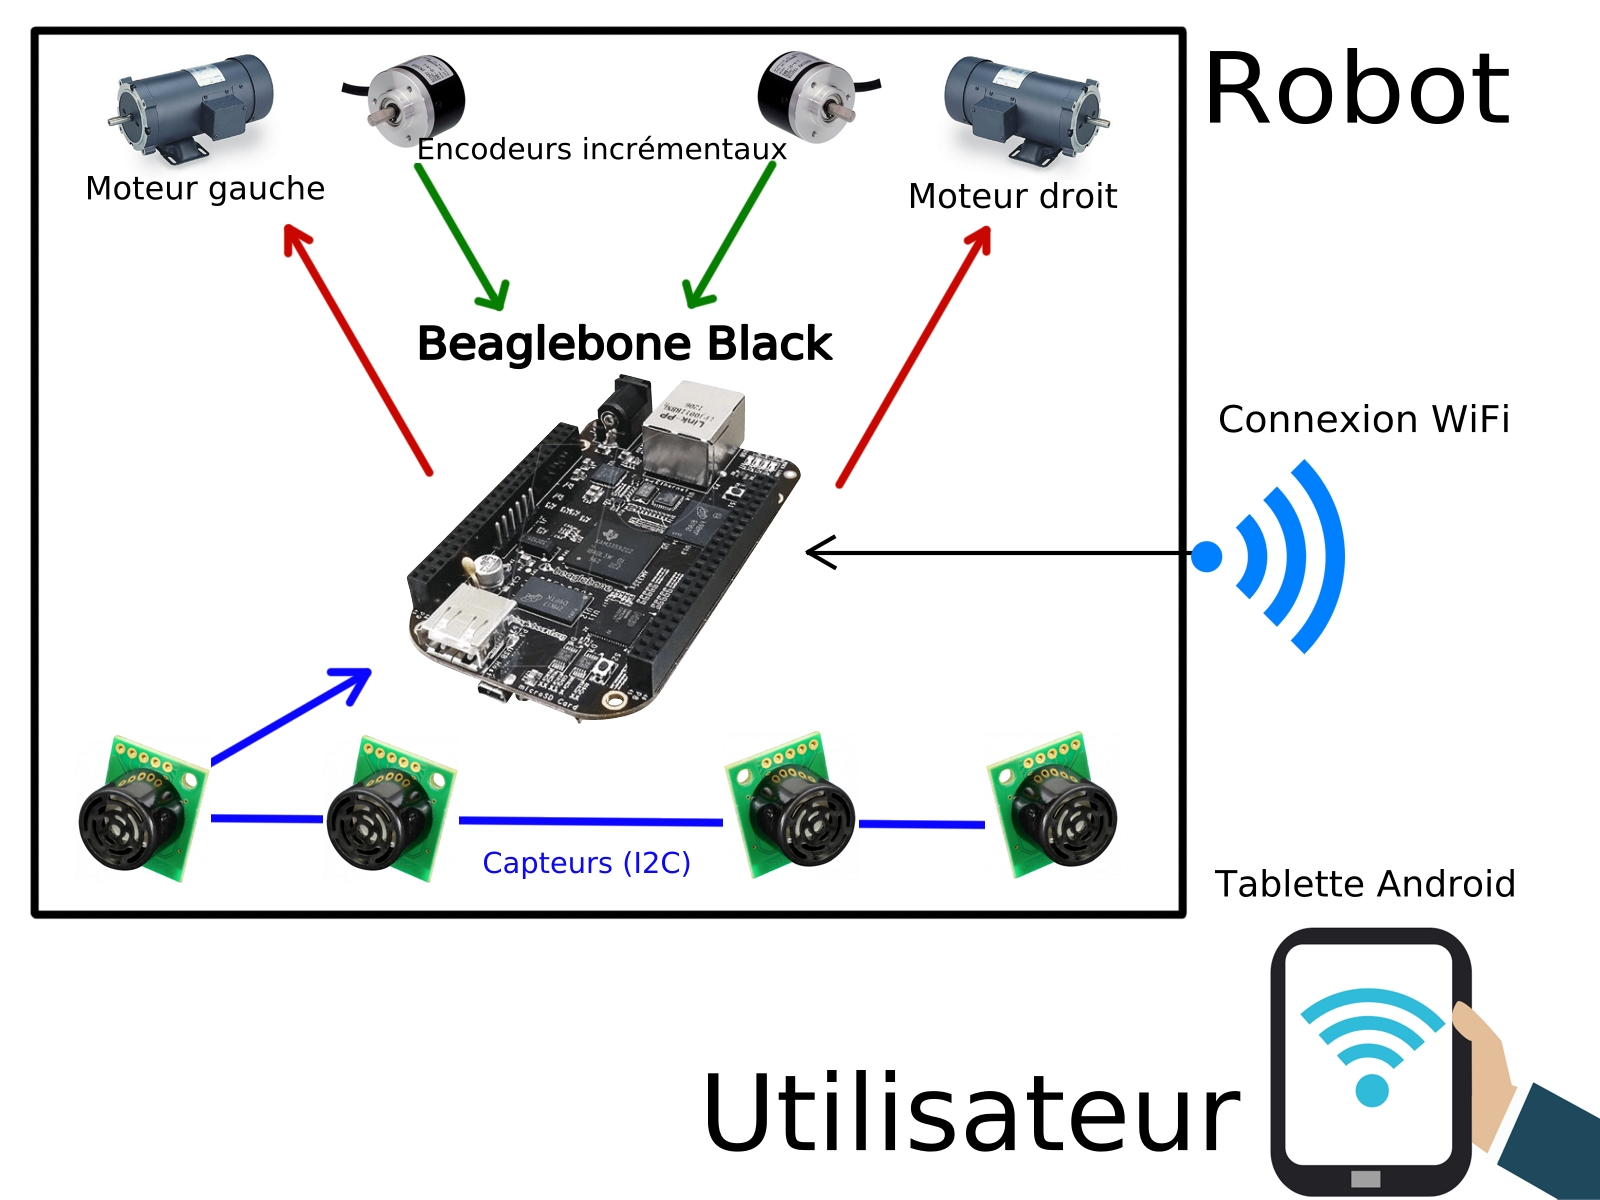
\includegraphics[scale=0.8]{img/hermes-archi.jpg}
\end{center}

    {Cette architecture est axée autour de deux éléments principaux :
    La Beaglebone Black, et la tablette Android.}

    \subsection{La Tablette Android}

    {La tablette Android est une des interfaces possibles pour l'interaction entre le robot
    et son utilisateur. En effet, il est également prévu de pouvoir contrôler le robot
    depuis une interface Web. Nous avions développé une application pour Android
    permettant le pilotage direct du robot (afin de tester le protocole de communication
    et la mobilité de la plateforme). Cependant, il s'agissait de la seule forme d'interaction
    possible en utilisant la tablette embarquée, ce qui était assez limité, et ne permettait
     pas encore le guidage d'un utilisateur dans le campus.}

     \subsection{Le choix de l'architecture matérielle embarquée}

     {Notre architecture avait pour objectif de tester les capacités d'un
     micro-ordinateur embarqué, afin de savoir si il était possible de gérer
     tous les éléments de base d'un robot depuis une unique carte. En effet,
     la plupart des architectures de robots que nous avions expérimenté pour l'instant
     (notamment au club de robotique de l'école) étaient constituées d'une carte
     dite "Bas niveau" et d'une carte dite "Haut Niveau". La première, souvent une carte
     de type Arduino, STM32, ou encore Teensy, avait pour rôle de gérer les
     problématiques de pilotage des moteurs et servomoteurs, tandis que la seconde
     permettait de gérer les problématiques de l'environnement du robot (grâce à l'interprétation
     des valeurs des capteurs) ainsi que la recherche de chemin (algorithme de Path Finding),
     mais aussi la communication avec l'utilisateur. Cette dernière, plus puissante,
     était souvent une Raspberry Pi. Cela nous obligeait donc à avoir
     un système de communication entre ces deux cartes, qu'il s'agisse d'une liaison série
     ou d'une connexion ethernet, transportant un protocole de communication simple réalisé
     par nos soins. Cependant, nous avions constaté des faiblesses qui pouvaient s'avérer
     critiques lorsque des déconnexions apparaissaient. Pour cette raison, nous voulions
     tester une autre forme d'architecture, en utilisant une seule et unique carte pour
     les applications haut et bas niveau.}

     \subsubsection{Fonctionnalités indispensables}

     {Afin de choisir l'ordinateur utilisé, nous avions deux contraintes principales :
     tout d'abord, la carte devait être suffisamment puissante pour permettre
     d'accueuillir des programmes "haut niveau" tels qu'un algorithme de recherche de chemin
     (relativement coûteux en terme de puissance de calcul) ou encore différents
     serveurs, comme par exemple notre serveur python en charge du traitement des
     phrases de la reconnaissance vocale. Tout cela fonctionnant en simultané avec
     le programme responsable de l'asservissement du robot, lui aussi potentiellement
     gourmand en ressources de calcul, de par la fréquence d'asservissement qui se doit
     d'être suffisamment élevée pour permettre de bons déplacements de la plate forme.
     Aussi, cette première contrainte nous obligeait à utiliser un système d'exploitation
     permettant d'installer et d'executer des programmes complexes et divers. C'est pour
     cela (et parce que nous le connaissions suffisamment) que nous avions choisi
     d'utiliser Linux.}
     {Puis, il fallait que la carte électronique possède les fonctionnalités
     hardwares indispensables pour pouvoir l'interfacer directement avec notre matériel,
     et en particulier avec les encodeurs incrémentaux permettant de mesurer la
     vitesse et la distance parcourue par le robot. En effet, ces systèmes ont pour
     sortie un signal dont nous devons pouvoir déduire le déplacement du robot en
     comptant simplement des fronts montants. Hors, ces fronts montants
     doivent êtres dénombrés grâce à des interruptions, il nous fallait donc choisir
     une carte embarquée disposant de gestion d'interruptions. Après quelques recherches,
     nous avions choisi d'utiliser une carte de type BeagleBone Black.}

     \subsubsection{La BeagleBone Black}

     {La carte Beaglebone black est un micro ordinateur destiné à être embarqué.
     Elle permet en théorie d'utiliser toutes les fonctionnalités requises par notre
     cahier des charges simultanément. Le processeur utilisé est un ARM Cortex A8
     cadencé à 1GHz, auquel on associe 512 Mo cd mémoire RAM DDR3, ce qui lui apporte
     des capacités de calcul supérieures à une Raspberry Pi. De plus, cette carte
     est plus adaptée à être utilisée dans des projets embarqués : elle possède
     beaucoup plus de GPIO, dont par exemple 3 bus I2C différents, contre un seul
     pour la Raspberry Pi 3. Dans la configuration actuelle du projet, un seul bus I2C
     peut suffir, cependant nous avions pensé à différentes améliorations qui pourraient
     demander des bus supplémentaires, ou davantage de GPIO.
     Enfin, la différence majeure avec une Raspberry Pi est que la Beaglebone
     possède des PRU (Programmable Real-Time Unit). Il s'agit en réalité de petits
     micro-controlleurs 32 bits indépendants situés dans la puce processeur de la carte,
     et qui permettent de faire cohabiter des fonctionnalités nécessitant du temps réel et un
     système d'exploitation qui ne l'est pas, dans notre cas, Linux. C'est cette différence
     fondamentale qui fait de la BeagleBone Black une carte bien plus adaptée à jouer
     le rôle d'ordinateur central unique pour un système robotisé.}

     \begin{center}
       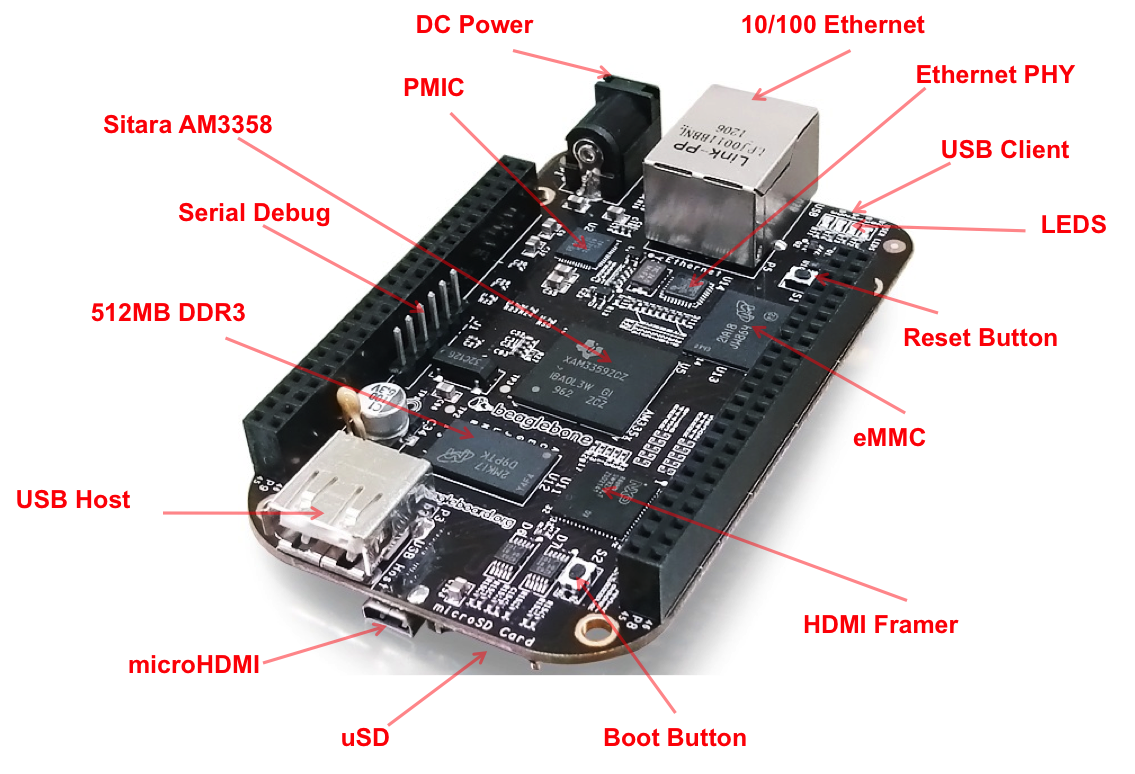
\includegraphics[scale=0.8]{img/black_hardware_details.png}
     \end{center}

     \subsection{L'architecture logicielle}

     \subsubsection{Le projet Yocto}
     {Comme nous souhaitions utiliser un système d'exploitation Linux, nous devions
     choisir quelle distribution de cet OS nous allions utiliser. Nous avions trois
     possibilités :}
     \begin{itemize}
       \item Utiliser une distribution Linux existante
       \item Utiliser un kernel Linux seul et installer manuellement les composants logiciels nécessaires
       \item Utiliser un outil de génération de distribution Linux personnalisée
     \end{itemize}

     La première option possédait des avantages (comme l'accès à des mises à jour, ou
     un meilleur support). Cependant, nous voulions essayer autant que possible d'utiliser
     un système minimaliste, afin de ne pas le surcharger avec des applications
     inutiles dans le cadre de notre projet. La seconde option pouvait nous mener
     vers une distribution personnalisée et minimaliste. Cependant, elle peut être
     très difficile à mettre en place, et n'est pas facilement reproductible (en cas
     de souci, il faudrait refaire une installation complète). Nous avons donc opté
     pour la dernière solution, c'est à dire l'utilisation d'un outil de génération de
     distributions adaptées aux systèmes embarqués comme le notre. Pour cela, nous avons
     utilisé l'outil Yocto.
     \newline
     Yocto est un projet communautaire contenant de nombreux outils et briques
     logicielles permettant de créer sa propre distribution Linux, adaptée
     au hardware tout en restant minimaliste. Yocto fonctionne sous forme de
     "recipes" (comprendre "recettes") qui, à la manière de recettes de
     cuisine, indiquent à la compilation où se procurer les sources d'un programme,
     comment le compiler, et où l'incorporer dans le système de fichier généré.
     En effet, Yocto utilise ces "recipes" pour générer une image binaire brute
     destinée à être directement copiée dans la mémoire de la carte embarquée (une
     carte micro SD dans notre cas).

    \section{Objectif du Projet de fin d'études}

    {L'objectif du PFE était de se focaliser davantage sur l'interaction directe
     entre les utilisateurs et le robot. Afin de pouvoir servir de guide, il
     fallait que le robot puisse recevoir des requêtes (de la forme "guide
     moi à l'amphi 10") de la manière la plus naturelle qui soit. Pour cela,
     nous avions choisi dans le cahier des charges d'utiliser une tablette
     tactile posée sur le robot. De plus, le projet devait rendre la base
     roulante utilisable en complétant les fonctionnalités qui n'avaient pas
     été implémentées lors du Cassiopée, en particulier la gestion des capteurs,
     et en tentant de corriger les anomalies constatées lors des tests à la fin
     du projet Cassiopée.}



  \chapter{Déroulement du PFE}

    \section{Intégration des capteurs}

    {Une des fonctionnalités prévues initialement dans le cahier des charges qui n'avait
    pas encore été implémentée lors du projet Cassiopée était la gestion des capteurs.
    Nous avions prévu de placer des capteurs ultrason à des endroits stratégiques du
    chassis du robot. En effet, la plateforme est sensée pouvoir se déplacer
    dans un environnement où des personnes peuvent gêner son mouvement. Hors, sans
    autre forme d'information sur son environnement, le robot ne peut pas prévoir
    là où se trouveront d'éventuels obstacles au moment où il planifie son trajet d'un
    point A à un point B. Il faut donc au minimum lui ajouter un "dispositif d'urgence",
    capable d'interrompre un déplacement si celui ci est perturbé par un obstacle
    inattendu.}

        \subsection{Description des capteurs}
        {Afin de détecter les obstacles das l'environnement proche du robot, nous
        avions choisi d'utiliser des capteurs à ultrason de type SRF02.}

        \begin{center}
          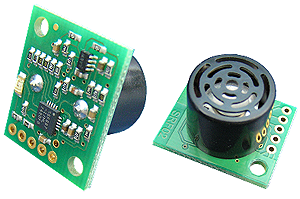
\includegraphics[scale=0.6]{img/srf02.png}
        \end{center}

        {Ces capteurs ont une portée de fonctionnement située entre 20cm et 240cm
        environ. Cette distance assez élevée permet, grâce à 5 capteurs répartis
        autour du robot, d'avoir une information minimale sur son environnement. Les
        capteurs à ultrason sont particulièrement adapté à ce type d'usage, puisqu'ils
        ont la particularité d'être très peu directifs. La disposition choisie était
        la suivante :}

        \begin{itemize}
          \item Un capteur vers l'arrière
          \item Un capteur sur chaque flanc
          \item Deux capteurs sur la face avant
        \end{itemize}

        {Ces capteurs peuvent fonctionner dans deux protocoles de communication
        différents : en liaison série RS232, ou en I2C. J'ai donc choisi d'utiliser le
        protocole I2C, afin d'utiliser les ports I2C inclus sur la Beaglebone Black, et
         ainsi découvrir le principe de fonctionnement de ce protocole. L'I2C est un
         protocole adapté à la communication entre plusieurs cartes électroniques
        peu éloignées les unes des autres. De plus, il se présente sous la forme d'un
        bus de communication dans lequel chaque capteur possède une adresse afin de
        pouvoir communiquer précisément avec lui. Cela rentrait tout à fait dans le cadre
        d'utilisation de ces capteurs sur le robot Hermes.}

        {Les Srf02 possèdent plusieurs fonctions pouvant être utilisées
        en leur envoyant des octets spécifiques. Parmi les fonctionnalités
        indispensable, on retrouve par exemple la fonction de rafraîchissement
        de la valeur de distance mesurée par le capteur. En effet, il ne réalise
        pas de mesure par lui même : il faut demander explicitement au capteur
        de refaire une mesure. Puis, la valeur mesurée est stockée dans un des
        registres du capteur. Une autre commande permet de récupérer la valeur
        stockée dans ce registre, dans différentes unités, ce qui m'a permis
        d'utiliser directement les valeurs en centimètres.}

        \subsection{Mise en application}

        {Les capteurs Srf02 sont des capteurs très répandus dans la communauté des
        "makers", en particulier des utilisateurs de cartes Arduino. Ils sont
        une véritable référence, grâce à leur facilité d'utilisation sur Arduino et
        grâce à leur prix assez faible (moins d'une vingtaine d'euros par capteur).
        Cependant, ils sont beaucoup moins utilisés sur des cartes plus puissantes, et
        en particulier des cartes embarquant un système d'exploitation Linux. Pour
        cette raison, je n'ai pas trouvé de bibliothèque permettant de les utiliser
        directement dans notre système d'exploitation Linux. En utilisant les informations
        fournies par le constructeur, j'ai néanmoins pu réaliser ma propre bibliothèque
        de fonctions. Ce code a été réalisé en C++ puisque le système de capteurs devait être
        intégré au programme "hermes-pilot", responsable des déplacements du robot, lui même
        codé en C++.}
        {Puis, une fois la bibliothèque préparée, il fallait réussir à utiliser les cinq
        capteurs en simultané. Pour cela, j'ai choisi d'opter pour la logique suivante :\newline
        Chacun des capteurs doit rafraîchir sa valeur avant de pouvoir envoyer une
        mesure. Hors, d'après la documentation du constructeur, il ne faut pas tenter
        de réaliser deux mesures avec moins de 65ms, car des valeurs absurdes pourraient
        apparaître si des ondes ultrasonores du premier capteur ne se sont pas estompées
        avant la mesure du second. Pour satisfaire cette exigeance, il fallait donc
        interroger chaque capteur de manière circulaire autour du robot, tout en
        attendant bien 65ms au minimum entre deux mesures. L'objectif était d'intégrer
        ce système de mise à jour des valeurs mesurées par les capteurs dans un thread
        du programme de pilotage du robot, et ainsi permettre au thread responsable
        du déplacement de consulter régulièrement les distances des obstacles éventuels,
        et réagir au plus vite en cas de potentielle collision.
        }


    \section{Développement et intégration du contrôle vocal}

      {Afin de rendre les communication avec le robot les plus naturelles possible
      pour les utilisateurs, nous avons choisi d'utiliser de la reconnaissance vocale.
      Le fonctionnement du système de reconnaissance vocale est organisé selon
      un modèle client - serveur :}

      \subsection{Le client}
      {Le client que nous avons développé est une application Android. Ce choix n'est
      pas arbitraire, il permet en effet d'offrir des fonctionnalités particulièrement
      intéressantes :}

        \subsubsection{La simplicité de l'interaction}
        {L'utilisation d'une tablette, qu'elle soit accompagnée ou non de reconnaissance
        vocale, était déjà prévue au début du projet Hermes. En effet, elle permet
        d'obtenir une forme d'interaction simple pour l'utilisateur grâce à son écran tactile.
        Celui ci devait permettre notamment de montrer une carte du lieu, ainsi qu'un écran
        pour rechercher le bureau d'une personne sur le campus simplement à partir de son
        nom.}

        \subsubsection{L'API de Google}
        {Nous avons choisi d'utiliser une tablette sous Android, pour la simplicité de
        développement que cela implique, mais aussi pour avoir l'accès à l'API de reconnaissance
        vocale de Google. Cette API est composée de deux éléments complémentaires :}
        \begin{itemize}
          \item Le STT (Speech to text) : c'est l'outil capable de traduire le fichier
          audio contenant la requête vocale de l'utilisateur en une requête sous forme de
          chaîne de caractères.
          \item Le TTS (Text To Speech) : il s'agit de l'outil faisant le travail inverse.
          À partir d'une chaîne de caractères, le TTS génère un fichier audio contenant une
          voix synthétisée lisant la chaîne de caractères.
        \end{itemize}

        {L'avantage dans notre cas est que Google fournit cette API dans tous les appareils
        Android, et qu'elle peut, en cas de déconnexion, être utilisée sans connexion Internet
         (ce qui était parfait dans notre cas, puisqu'il fallait que le mode d'interaction
         avec le robot ne soit pas tributaire de la présence d'une connexion wifi ou non).}

    \section{Le serveur}

    {Une fois que le client sur la tablette Android a traduit la phrase prononcée
    par l'utilisateur en chaîne de caractères, elle est envoyée sur le serveur
    hébergé sur la Beaglebone Black. Puis, le serveur procède à l'interprétation
    de cette phrase et est chargé de renvoyer une réponse au client, qui sera
    prononcée à haute voix par la tablette. Le processus d'analyse des phrases
    a été entièrement créé, testé, puis intégré dans le robot.}

    \section{Compréhension et génération de réponses}
    {N'ayant que trop peu de connaissances sur les réseaux de neurones, et un cahier des
    charges pouvant être respecté grâce à un modèle "rule-based", j'ai réalisé
    le programme serveur en suivant une architecture proche de celle d'un projet
    Open Source nommé Mycroft (ayant une fonction assez similaire), codé en Python 3.}
      \subsection{Les "Skills"}
      {Afin de rendre l'assistant très modulaire et ainsi simplifier la gestion des phrases
      auxquelles il sait répondre, j'ai gardé le concept de "Skills" du projet Mycroft.
      Un Skill est tout simplement un morceau de code que l'on peut importer dans le coeur
       du programme serveur, afin d'ajouter des phrases au dictionnaire de requêtes connues
        et leur associer une fonction de réponse.\newline}
      {Ce programme étant orienté objet, j'ai créé des classes possédant les
      spécifications suivantes :\newline\newline}

      \subsubsection{La classe Skill}

        {Les attributs :}
        \begin{itemize}
          \item \textbf{keyPhrases} : la liste des phrases exactes connues. Par exemple, ["Quelle heure est-il ?", "Il est quelle heure ?"]
          \item \textbf{superWords} : Liste de mots ou motifs de mots clés permettant d'interpréter une phrase qui n'est pas dans keyPhrases. Dans notre exemple, ["heure", "quelle heure"]
          \item \textbf{badWords} : Liste "anti mots clés", contient des mots ou motifs qui nous montrent qu'il ne faut pas interpréter la phrase. Dans notre exemple, ["à quelle heure"]
          \item \textbf{result} : C'est la fonction à exécuter si la requête est confirmée comme étant un appel à ce skill. Dans notre exemple, il s'agit d'une fonction qui demandera l'heure au système d'exploitation, et la renverra sous la forme d'une chaîne de caractères telle que "Il est XX heures et XX minutes".
          \item \textbf{keyWords} \textit{(attribut dérivé)} : Il s'agit d'un dictionnaire des mots contenus dans les keyPhrases. il est généré à la construction de l'objet en décomposant chaque keyPhrase. Pour notre exemple, il vaudra ["quelle", "heure", "est", "il"] (on retire les mots en doublon)\newline
        \end{itemize}
        {Les méthodes :}
        \begin{itemize}
          \item \textbf{ask} : Méthode qui prend en argument la requête, et qui vérifie si la question posée par l'utilisateur est dans les keyPhrases. Renvoie un booléen.
          \item \textbf{similitude} : Méthode qui prend en argument la requête, et qui attribue à la requête un score en fonction de la "similitude" avec les keyPhrases, la présence de superWords ou de badWords. Les paramètres du calcul sont modifiables, par exemple, on a choisi d'attribuer +1 au score pour chaque keyWord présent dans la requête, +20 pour un superWord, et -40 pour un badWord. La fonction renvoie dont un entier représentant le score de similitude.
          \item \textbf{execute} : Méthode qui execute le Skill lorsqu'il est confirmé (c'est à dire qu'il appelle la fonction fournie pour result)\newline
        \end{itemize}

        {Comme nous l'avons vu avec l'exemple de la demande d'heure, la classe Skill permet de
        définir une capacité générique pour l'assistant vocal. Elle permet une simple association
        requête \textrightarrow \space fonction à éxécuter. C'est donc le modèle de Skill que
         nous utilisons pour la plupart des fonctionnalités ne demandant pas un traitement plus
          complexe.}
        {Cependant, cela semblait intéressant de créer deux classes filles afin de s'adapter
        aux fonctionnalités plus spécifiques. Il s'agit des classes TextSkill et ArgSkill.}
      \subsubsection{La classe TextSkill}
        {De nombreuses requêtes ont pour réponse une simple phrase. Par exemple, si l'on demande
        au robot \textit{"qui es tu ?"} il pourra tout simplement répondre par une phrase connue
         à l'avance : \textit{"Je suis le robot Hermes"}. il fallait donc créer une classe
         spécifique pour ce type de requêtes.\newline}
        {Pour rendre l'interaction avec le robot plus authentique, il fallait
        que pour chaque question de l'utilisateur, le robot possède plusieurs réponses
        formulées différemment. Une de ces réponses est choisie aléatoirement avant d'être
         renvoyée.\newline}
        {La différence entre un Skill et un TextSkill est que la fonction \textit{return}
        est déjà connue pour un TextSkill : il s'agit du retour aléatoire d'un élément
        d'une liste de réponses connues. Cependant, si il ne faut plus fournir une
        fonction \textit{return} dans le constructeur d'un TextSkill, il faut tout de
        même lui fournir la liste des réponses que l'on souhaite affecter à la requête.}
      \subsubsection{La classe ArgSkill}
        {Cette classe a été créée pour les Skills les plus complexes. En effet, il
        fallait que l'assistant puisse comprendre une requête contenant un "argument",
        comme par exemple la phrase \textit{"Guide moi au bâtiment B"}. Pour cela,
        il doit être capable de décomposer la phrase en deux partie : la requête
        (\textit{"Guide moi à"}) et l'argument (\textit{"bâtiment B"}). Puis, il doit
        appeler le Skill correspondant à la requête \textit{"Guide moi à"}, en lui
        fournissant l'argument du lieu où l'on doit guider, afin de pouvoir envoyer
         une requête de Path Finding vers l'endroit demandé au programme responsable
          du déplacement du robot.\newline}
        {Ainsi, la différence fondamentale entre le Skill et le ArgSkill, est qu'un
         ArgSkill possède une fonction \textit{return} qui demande qu'on lui fournisse
        la requête de l'utilisateur afin de pouvoir en extraire l'argument et l'utiliser.
        De plus, un ArgSkill possède une méthode \textit{ask} modifiée : en effet,
        on ne vérifie pas que la requête corresponde parfaitement à une keyPhrase connue,
        mais on vérifie à la place que la keyPhrase connue (par exemple \textit{"Guide moi à"})
        est \textbf{inclue} dans la requête. Sans cela, nous ne pourrions jamais identifier
        précisément les requêtes, puisque l'argument n'est pas connu à l'avance.}


    \subsection{Le package core}
    {Le package core contient l'essentiel de ce qui est à importer pour pouvoir utiliser
     le coeur du système. En effet, importer le fichier core.py suffit à créer tous
     les objets Skills, et il contient la fonction principale du programme que j'ai
     appelé \textit{executeOrder(order)}. Cette fonction demande l'ordre envoyé en argument,
      et se charge d'interroger les Skills, afin de trouver celui qui correspond le
       mieux à la requête faite par l'utilisateur, avant de l'éxécuter. Bien entendu,
       l'interrogation des différents Skills se fait d'une manière précise :}
      \subsubsection{Première vérification}
      {Dès que la fonction \textit{executeOrder} est appelée, le programme récupère la
       requête de l'utilisateur. Il va commencer par la "première vérification".
       Pour limiter au maximum la complexité (et donc le temps de réponse) du programme,
        la première vérification consiste à utiliser la méthode \textit{ask} sur
         chacun des Skills instanciés. On vérifie donc si la phrase prononcée
         par l'utilisateur fait partie des phrases connues (il faut que la requête
         soit \textbf{exactement} une keyPhrase).\newline}
      {Si la requête est trouvée parmi les keyPhrases d'un Skill,
      alors on lance l'éxécution de ce Skill. Cependant, si la phrase n'est
      pas connue au mot près, on passe à la seconde vérification, plus fine mais
      qui demande plus de calculs.}
      \subsubsection{Seconde vérification}
      {Si la première vérification a échouée, on doit procéder à une analyse plus
      fine de la requête de l'utilisateur. C'est à ce moment qu'intervient la
      méthode \textit{similitude} des Skills. En effet, le programme va demander
      à chaque Skill son "score de ressemblance" avec la requête. Cela revient
      en somme à un calcul de la probablilité que la requête corresponde bien au
      Skill interrogé. Une fois que chaque Skill a calculé son score, l'algorithme
      repère le Skill qui a obtenu le meilleur score. Cependant, nous ne pouvons
      pas dire que ce Skill correspond bien à ce qui a été demandé par l'utilisateur !
       Par exemple, si le meilleur score est de 1 (et donc que tous les autres sont de 0)
        cela signifiera qu'un mot banal (par exemple \textit{"il"}) était commun entre
        la requête et une des phrases connues dans le Skill. Cela ne permet en aucun cas
         de dire que la question de l'utilisateur était \textit{"quelle heure est il ?"}, parce
         que la le score est trop faible. Il fallait donc fixer arbitrairement un seuil, un score
          minimum, à partir duquel il est possible d'envisager que le Skill ayant
          le plus grand score corresponde bien ce que l'utilisateur a demandé. Cependant,
          si deux Skills obtiennent un score très élevé, mais trop proches l'un de l'autre,
           on supposera que l'on ne peut pas distinguer lequel des deux est le plus probable.
           J'ai donc choisi arbitrairement un second seuil correspondant à l'écart de score
           minimal à respecter entre le Skill de score maximal et le second afin de valider
           le premier.}
      {En résumé, pour qu'un Skill soit validé à la seconde vérification, il faut :}
      \begin{itemize}
        \item Qu'il soit celui qui obtient le score maximal
        \item Que son score soit au dessus d'un seuil minimal
        \item Que l'écart entre son score et le second plus haut score dépasse un certain seuil
      \end{itemize}
      {Si ces trois conditions sont validées, alors l'algorithme déterminera qu'il est très
      probable que la requête de l'utilisateur corresponde à ce à quoi le Skill peut répondre,
      et lancera son éxécution. Après avoir essayé différentes valeurs pour les seuils
      arbitraires ainsi que pour les points que rapportent les mots clés et anti mots clés,
      on peut trouver un compromis intéressant qui est capable de répondre à une requête
      dont la forme est inconnue du système au préalable.}

    \subsection{Le protocole de communication Client-Serveur}

    {Comme l'architecture choisie était une architecture Client - Serveur, il
    fallait également prévoir un protocole de communication entre les deux programmes.}

      \subsubsection{Fonctionnement du serveur}
        {Pour éviter certains blocages qui pouvaient apparaître (par exemple quand
        le serveur demande une confirmation à l'utilisateur, comme "Voulez vous
        vraiment que je vous amène au Bâtiment C ?"), il était préférable de coder
        ce programme serveur en mode "stateless". Cela signifie que le serveur
        n'aura aucune information stockée sur l'état du client. Grâce à ce système,
        lorsque l'on demande une confirmation, le serveur n'est pas bloqué à attendre
        une réponse à la confirmation. Il attendra tout simplement un message comme
        les autres, qui pourra soit être une requête qui n'a rien à voir, soit la
        même requête que précédemment mais avec un petit indicateur pour dire que
        le client l'a confirmé.}

      \subsubsection{Gestion des sockets}
        {Afin de permettre la communication entre le client et le serveur, j'ai choisi
        d'utiliser des sockets en TCP, afin de profiter de tous les avantages de ce
        protocole (acquittements, reprise sur perte...)\newline}
        {Comme le serveur est "stateless", il possède simplement un socket qui
        écoute sur un port et attend de recevoir une connexion et un message.
        Il répondra au client tant que la connexion est encore ouverte, puis
        fermera la connexion, et se remettra en attente.\newline}
        {De son côté, le client se connectera au serveur pour envoyer sa requête,
        attendra la réponse, et fermera la connexion. Et ce, pour chaque requête
        émise par l'utilisateur.}

      \subsubsection{Format des messages échangés}

        {Puisque le seveur et le client utilisent des deux côtés des langages de
        programmation objet
        haut niveau, il était possible d'utiliser des messages au format JSON.
        Les messages JSON ont la particularité d'être directement interprétables
        en tant qu'objets, ce qui simplifie grandement le traitement des messages
        contenant plusieurs informations
        simultanées.\newline}


        {Voici un exemple de requête JSON envoyée par le client :}
        \begin{listing}[h]
          \begin{minted}[frame=single,
                         framesep=3mm,
                         linenos=true,
                         xleftmargin=21pt,
                         tabsize=4]{js}
{
  "type": "question",
  "msg": "Quelle heure est-il ?"
}
          \end{minted}
        \end{listing}

        {Cet exemple correspond à une simple question, sans particularité, et elle
        aura pour réponse (après traitement par le serveur) un JSON de la forme :}

        \begin{listing}[h]
          \begin{minted}[frame=single,
                         framesep=3mm,
                         linenos=true,
                         xleftmargin=21pt,
                         tabsize=4]{js}
{
  "type": "answer",
  "msg": "Il est 08 heures et 45 minutes."
}
          \end{minted}
        \end{listing}

        {Cependant, il existe des requêtes qui demandent une confirmation à
        l'utilisateur, afin d'être sûrs d'avoir bien compris ce qu'il demandait.
        Pour cela, il suffit d'utiliser d'autres champs JSON,
        en suivant le schéma suivant :}

        \newpage

        \begin{listing}[h]
          \begin{minted}[frame=single,
                         framesep=3mm,
                         linenos=true,
                         xleftmargin=21pt,
                         tabsize=4]{js}
{
  "type": "question",
  "msg": "Amène moi en Amphi 10"
}
          \end{minted}
          \title{Etape 1 : Requête de l'utilisateur}
        \end{listing}
        \begin{listing}[h]
          \begin{minted}[frame=single,
                         framesep=3mm,
                         linenos=true,
                         xleftmargin=21pt,
                         tabsize=4]{js}
{
  "type": "askConfirmation",
  "msg": "Voulez vous que je vous amène à Amphi 10 ?",
  "originalRequest": "Amène moi en Amphi 10"
}
          \end{minted}
          \title{Etape 2 : Réponse du serveur (demande de confirmation)}

          \begin{minted}[frame=single,
                         framesep=3mm,
                         linenos=true,
                         xleftmargin=21pt,
                         tabsize=4]{js}
{
  "type": "confirmation",
  "msg": "Amène moi en Amphi 10",
  "answer": "Oui"
}
          \end{minted}
          \title{Etape 3 : Confirmation de l'utilisateur}

          \begin{minted}[frame=single,
                         framesep=3mm,
                         linenos=true,
                         xleftmargin=21pt,
                         tabsize=4]{js}
{
  "type": "answer",
  "msg": "OK, je vous guide à Amphi 10."
}
          \end{minted}
          \title{Etape 4 : Réponse finale du serveur}
        \end{listing}


\subsection{Intégration dans la distribution Linux}
{Pour permettre l'intégration de ce serveur dans la distribution Linux, il fallait
commencer par rendre possible son exécution dans cet environnement en satisfaisant
au préalable toutes ses dépendances envers d'autres logiciels. En priorité, il
fallait ajouter le support de Python version 3. En effet, par défaut, notre distribution
Linux ne contenait que Python 2.7 qui ne permettait pas d'exécuter le code du serveur
hermes-vocal. Pour se faire, il a fallu ajouter la "recipe" (donc la recette de
compilation) de Python 3 dans la liste des fichiers de notre projet Yocto. Puis, il
a fallu ajouter également deux bibliothèques python : le module "wikipedia", permettant,
comme son nom l'indique, de réaliser des recherches sur Wikipédia, ainsi que le module
"psutil", permettant de récupérer des informations sur le système (charge CPU, pourcentage
de mémoire RAM utilisée...). Pour cela, il était plus simple d'ajouter dans le projet
Yocto l'installeur de modules "pip" et de l'utiliser pour ajouter les modules nécessaires.
Puis, il fallait cloner le dépot git contenant le code du serveur afin de pouvoir
le lancer.}


\chapter{Bilan du projet}
\section{Problèmes rencontrés}
\subsubsection{Yocto}
{Aussi intéressant et performant qu'il soit, Yocto reste un projet communautaire assez
jeune. Cela a pour conséquence de lui donner un caractère assez "instable" dans son
développement, et peut parfois mener à des pertes de temps considérables. En effet,
au début du projet de fin d'études, il fallait mettre à jour le système Yocto existant, à cause
d'incompatibilités entre plusieurs "Layers" de Yocto. Les "Layers" sont des groupements
de recettes de compilation. Notre projet contient par exemple, entre autre, un layer spécialement
pour le support de la Beaglebone Black, mais aussi un layer personnalisé pour ajouter
nos programmes (hermes-pilot et hermes-vocal par exemple). Hors, lors de cette mise
à jour, certaines fonctionnalités essentielles sur Beaglebone Black ont disparu sans
être remplacées ! Dans mon cas, il s'agissait de la gestion des PWM (permettant la
commande des moteurs de propulsion). }

\subsubsection{La plateforme du projet Cassiopée}
{Le projet, bien que relativement abouti sur le plan de l'interface homme-machine
ainsi que sur l'intégration des capteurs s'est légèrement éloigné de l'objectif final
fixé lors de la proposition du projet. En effet, je pensais pouvoir faire fonctionner
la plateforme créée lors du projet Cassiopée afin de pouvoir tester la validité
des fonctionnalités qui ont été implémentées. Hors, plusieurs problèmes se sont présentés,
et m'ont contraint à revoir ces ambitions à la baisse. En effet, la base du robot
n'avait été que très peu testée avec le reste de l'architecture lors du Cassiopée,
par faute de temps. Il restait quelques problèmes non résolus, notamment au sujet
des cartes élecroniques de puissance sensées alimenter les moteurs. Une de ces
deux cartes avait été détruite pour une raison inconnue (supposément une erreur
de branchement ou de manipulation) et avait donc dû être remplacée en urgence
par une carte de puissance différente fabriquée au laboratoire du département
Physique de l'école. Afin de rendre le système symétrique, j'avais
pour projet de réaliser une seconde carte similaire au laboratoire de physique,
ce qui fut fait. Mais entre temps, un souci électronique différent (et toujours
d'origine indéterminée) a fait que j'ai détruit une Beaglebone Black en tentant
de faire fonctionner les capteurs montés sur le robot. Cette erreur m'a couté
du temps, et ne m'a laissé que deux solutions : chercher à trouver précisément la
source de ce problème, ou continuer à me concentrer sur les fonctionnalités
implémentées afin de les tester sur un autre robot. C'est finalement la seconde option
qui a été retenue, faute de temps encore une fois. La démonstration de mon système
de contrôle vocal a donc été possible mais sur une autre plateforme miniaturisée
ayant déjà servie de plateforme de tests lors du projet Cassiopée.}

\section{Conclusion}
{Ce projet a été pour moi l'occasion de me confronter à divers problèmes et
de découvrir des technologies très variées. Allant de l'électronique, voire même
de la mécanique, jusqu'à de la reconnaissance vocale, il faut reconnaître que ce
projet était particulièrement diversifié. Cela lui a donné toute sa dimension
passionnante, mais aussi complexe. En effet, l'idée à l'origine du projet est
particulièrement ambitieuse : de nombreuses équipes d'ingénieurs de différentes
entreprises de robotique se sont attaqué à la conceptions de robots guides, et
on remarque encore assez peu de ces machines aujourd'hui. Mais il est intéressant
de noter que la réflexion autour de ce projet a été suffisamment bien menée pour
aboutir à plusieurs prototypes, physiques, électroniques, ou logiciels, qui peuvent
s'adapter à d'autres contextes. En particulier, le système de contrôle vocal
développé dans l'optique de diriger un robot pourrait être adapté au contrôle
d'un ordinateur quelconque, tant il est simple d'adapter ses fonctionnalités.
Même si le projet n'a pas encore abouti à une forme finale de robot guide, les
briques indépendantes conçues lors du projet Cassiopée puis de ce PFE démontrent
qu'il est possible de créer de toutes pièces des projets de ce niveau de complexité
au niveau de prototype sans pour autant disposer d'une équipe d'ingénieurs ou de
moyens très élevés.}



\end{document}
